% Options for packages loaded elsewhere
\PassOptionsToPackage{unicode}{hyperref}
\PassOptionsToPackage{hyphens}{url}
\PassOptionsToPackage{dvipsnames,svgnames,x11names}{xcolor}
%
\documentclass[
  single column]{article}

\usepackage{amsmath,amssymb}
\usepackage{iftex}
\ifPDFTeX
  \usepackage[T1]{fontenc}
  \usepackage[utf8]{inputenc}
  \usepackage{textcomp} % provide euro and other symbols
\else % if luatex or xetex
  \usepackage{unicode-math}
  \defaultfontfeatures{Scale=MatchLowercase}
  \defaultfontfeatures[\rmfamily]{Ligatures=TeX,Scale=1}
\fi
\usepackage[]{libertinus}
\ifPDFTeX\else  
    % xetex/luatex font selection
\fi
% Use upquote if available, for straight quotes in verbatim environments
\IfFileExists{upquote.sty}{\usepackage{upquote}}{}
\IfFileExists{microtype.sty}{% use microtype if available
  \usepackage[]{microtype}
  \UseMicrotypeSet[protrusion]{basicmath} % disable protrusion for tt fonts
}{}
\makeatletter
\@ifundefined{KOMAClassName}{% if non-KOMA class
  \IfFileExists{parskip.sty}{%
    \usepackage{parskip}
  }{% else
    \setlength{\parindent}{0pt}
    \setlength{\parskip}{6pt plus 2pt minus 1pt}}
}{% if KOMA class
  \KOMAoptions{parskip=half}}
\makeatother
\usepackage{xcolor}
\usepackage[top=30mm,left=25mm,heightrounded,headsep=22pt,headheight=11pt,footskip=33pt,ignorehead,ignorefoot]{geometry}
\setlength{\emergencystretch}{3em} % prevent overfull lines
\setcounter{secnumdepth}{-\maxdimen} % remove section numbering
% Make \paragraph and \subparagraph free-standing
\makeatletter
\ifx\paragraph\undefined\else
  \let\oldparagraph\paragraph
  \renewcommand{\paragraph}{
    \@ifstar
      \xxxParagraphStar
      \xxxParagraphNoStar
  }
  \newcommand{\xxxParagraphStar}[1]{\oldparagraph*{#1}\mbox{}}
  \newcommand{\xxxParagraphNoStar}[1]{\oldparagraph{#1}\mbox{}}
\fi
\ifx\subparagraph\undefined\else
  \let\oldsubparagraph\subparagraph
  \renewcommand{\subparagraph}{
    \@ifstar
      \xxxSubParagraphStar
      \xxxSubParagraphNoStar
  }
  \newcommand{\xxxSubParagraphStar}[1]{\oldsubparagraph*{#1}\mbox{}}
  \newcommand{\xxxSubParagraphNoStar}[1]{\oldsubparagraph{#1}\mbox{}}
\fi
\makeatother

\usepackage{color}
\usepackage{fancyvrb}
\newcommand{\VerbBar}{|}
\newcommand{\VERB}{\Verb[commandchars=\\\{\}]}
\DefineVerbatimEnvironment{Highlighting}{Verbatim}{commandchars=\\\{\}}
% Add ',fontsize=\small' for more characters per line
\usepackage{framed}
\definecolor{shadecolor}{RGB}{241,243,245}
\newenvironment{Shaded}{\begin{snugshade}}{\end{snugshade}}
\newcommand{\AlertTok}[1]{\textcolor[rgb]{0.68,0.00,0.00}{#1}}
\newcommand{\AnnotationTok}[1]{\textcolor[rgb]{0.37,0.37,0.37}{#1}}
\newcommand{\AttributeTok}[1]{\textcolor[rgb]{0.40,0.45,0.13}{#1}}
\newcommand{\BaseNTok}[1]{\textcolor[rgb]{0.68,0.00,0.00}{#1}}
\newcommand{\BuiltInTok}[1]{\textcolor[rgb]{0.00,0.23,0.31}{#1}}
\newcommand{\CharTok}[1]{\textcolor[rgb]{0.13,0.47,0.30}{#1}}
\newcommand{\CommentTok}[1]{\textcolor[rgb]{0.37,0.37,0.37}{#1}}
\newcommand{\CommentVarTok}[1]{\textcolor[rgb]{0.37,0.37,0.37}{\textit{#1}}}
\newcommand{\ConstantTok}[1]{\textcolor[rgb]{0.56,0.35,0.01}{#1}}
\newcommand{\ControlFlowTok}[1]{\textcolor[rgb]{0.00,0.23,0.31}{\textbf{#1}}}
\newcommand{\DataTypeTok}[1]{\textcolor[rgb]{0.68,0.00,0.00}{#1}}
\newcommand{\DecValTok}[1]{\textcolor[rgb]{0.68,0.00,0.00}{#1}}
\newcommand{\DocumentationTok}[1]{\textcolor[rgb]{0.37,0.37,0.37}{\textit{#1}}}
\newcommand{\ErrorTok}[1]{\textcolor[rgb]{0.68,0.00,0.00}{#1}}
\newcommand{\ExtensionTok}[1]{\textcolor[rgb]{0.00,0.23,0.31}{#1}}
\newcommand{\FloatTok}[1]{\textcolor[rgb]{0.68,0.00,0.00}{#1}}
\newcommand{\FunctionTok}[1]{\textcolor[rgb]{0.28,0.35,0.67}{#1}}
\newcommand{\ImportTok}[1]{\textcolor[rgb]{0.00,0.46,0.62}{#1}}
\newcommand{\InformationTok}[1]{\textcolor[rgb]{0.37,0.37,0.37}{#1}}
\newcommand{\KeywordTok}[1]{\textcolor[rgb]{0.00,0.23,0.31}{\textbf{#1}}}
\newcommand{\NormalTok}[1]{\textcolor[rgb]{0.00,0.23,0.31}{#1}}
\newcommand{\OperatorTok}[1]{\textcolor[rgb]{0.37,0.37,0.37}{#1}}
\newcommand{\OtherTok}[1]{\textcolor[rgb]{0.00,0.23,0.31}{#1}}
\newcommand{\PreprocessorTok}[1]{\textcolor[rgb]{0.68,0.00,0.00}{#1}}
\newcommand{\RegionMarkerTok}[1]{\textcolor[rgb]{0.00,0.23,0.31}{#1}}
\newcommand{\SpecialCharTok}[1]{\textcolor[rgb]{0.37,0.37,0.37}{#1}}
\newcommand{\SpecialStringTok}[1]{\textcolor[rgb]{0.13,0.47,0.30}{#1}}
\newcommand{\StringTok}[1]{\textcolor[rgb]{0.13,0.47,0.30}{#1}}
\newcommand{\VariableTok}[1]{\textcolor[rgb]{0.07,0.07,0.07}{#1}}
\newcommand{\VerbatimStringTok}[1]{\textcolor[rgb]{0.13,0.47,0.30}{#1}}
\newcommand{\WarningTok}[1]{\textcolor[rgb]{0.37,0.37,0.37}{\textit{#1}}}

\providecommand{\tightlist}{%
  \setlength{\itemsep}{0pt}\setlength{\parskip}{0pt}}\usepackage{longtable,booktabs,array}
\usepackage{calc} % for calculating minipage widths
% Correct order of tables after \paragraph or \subparagraph
\usepackage{etoolbox}
\makeatletter
\patchcmd\longtable{\par}{\if@noskipsec\mbox{}\fi\par}{}{}
\makeatother
% Allow footnotes in longtable head/foot
\IfFileExists{footnotehyper.sty}{\usepackage{footnotehyper}}{\usepackage{footnote}}
\makesavenoteenv{longtable}
\usepackage{graphicx}
\makeatletter
\def\maxwidth{\ifdim\Gin@nat@width>\linewidth\linewidth\else\Gin@nat@width\fi}
\def\maxheight{\ifdim\Gin@nat@height>\textheight\textheight\else\Gin@nat@height\fi}
\makeatother
% Scale images if necessary, so that they will not overflow the page
% margins by default, and it is still possible to overwrite the defaults
% using explicit options in \includegraphics[width, height, ...]{}
\setkeys{Gin}{width=\maxwidth,height=\maxheight,keepaspectratio}
% Set default figure placement to htbp
\makeatletter
\def\fps@figure{htbp}
\makeatother
% definitions for citeproc citations
\NewDocumentCommand\citeproctext{}{}
\NewDocumentCommand\citeproc{mm}{%
  \begingroup\def\citeproctext{#2}\cite{#1}\endgroup}
\makeatletter
 % allow citations to break across lines
 \let\@cite@ofmt\@firstofone
 % avoid brackets around text for \cite:
 \def\@biblabel#1{}
 \def\@cite#1#2{{#1\if@tempswa , #2\fi}}
\makeatother
\newlength{\cslhangindent}
\setlength{\cslhangindent}{1.5em}
\newlength{\csllabelwidth}
\setlength{\csllabelwidth}{3em}
\newenvironment{CSLReferences}[2] % #1 hanging-indent, #2 entry-spacing
 {\begin{list}{}{%
  \setlength{\itemindent}{0pt}
  \setlength{\leftmargin}{0pt}
  \setlength{\parsep}{0pt}
  % turn on hanging indent if param 1 is 1
  \ifodd #1
   \setlength{\leftmargin}{\cslhangindent}
   \setlength{\itemindent}{-1\cslhangindent}
  \fi
  % set entry spacing
  \setlength{\itemsep}{#2\baselineskip}}}
 {\end{list}}
\usepackage{calc}
\newcommand{\CSLBlock}[1]{\hfill\break\parbox[t]{\linewidth}{\strut\ignorespaces#1\strut}}
\newcommand{\CSLLeftMargin}[1]{\parbox[t]{\csllabelwidth}{\strut#1\strut}}
\newcommand{\CSLRightInline}[1]{\parbox[t]{\linewidth - \csllabelwidth}{\strut#1\strut}}
\newcommand{\CSLIndent}[1]{\hspace{\cslhangindent}#1}

\input{/Users/joseph/GIT/latex/latex-for-quarto.tex}
\makeatletter
\@ifpackageloaded{caption}{}{\usepackage{caption}}
\AtBeginDocument{%
\ifdefined\contentsname
  \renewcommand*\contentsname{Table of contents}
\else
  \newcommand\contentsname{Table of contents}
\fi
\ifdefined\listfigurename
  \renewcommand*\listfigurename{List of Figures}
\else
  \newcommand\listfigurename{List of Figures}
\fi
\ifdefined\listtablename
  \renewcommand*\listtablename{List of Tables}
\else
  \newcommand\listtablename{List of Tables}
\fi
\ifdefined\figurename
  \renewcommand*\figurename{Figure}
\else
  \newcommand\figurename{Figure}
\fi
\ifdefined\tablename
  \renewcommand*\tablename{Table}
\else
  \newcommand\tablename{Table}
\fi
}
\@ifpackageloaded{float}{}{\usepackage{float}}
\floatstyle{ruled}
\@ifundefined{c@chapter}{\newfloat{codelisting}{h}{lop}}{\newfloat{codelisting}{h}{lop}[chapter]}
\floatname{codelisting}{Listing}
\newcommand*\listoflistings{\listof{codelisting}{List of Listings}}
\makeatother
\makeatletter
\makeatother
\makeatletter
\@ifpackageloaded{caption}{}{\usepackage{caption}}
\@ifpackageloaded{subcaption}{}{\usepackage{subcaption}}
\makeatother
\ifLuaTeX
  \usepackage{selnolig}  % disable illegal ligatures
\fi
\usepackage{bookmark}

\IfFileExists{xurl.sty}{\usepackage{xurl}}{} % add URL line breaks if available
\urlstyle{same} % disable monospaced font for URLs
\hypersetup{
  pdftitle={Feedback on `Need for Speed? The role of perceptual speed in generalised visual comparison'},
  pdfauthor={Joseph A. Bulbulia},
  colorlinks=true,
  linkcolor={blue},
  filecolor={Maroon},
  citecolor={Blue},
  urlcolor={Blue},
  pdfcreator={LaTeX via pandoc}}

\title{Feedback on `Need for Speed? The role of perceptual speed in
generalised visual comparison'}

\usepackage{academicons}
\usepackage{xcolor}

  \author{Joseph A. Bulbulia}
            \affil{%
             \small{     Victoria University of Wellington, New Zealand
          ORCID \textcolor[HTML]{A6CE39}{\aiOrcid} ~0000-0002-5861-2056 }
              }
      


\date{2024-07-11}
\begin{document}
\maketitle

\subsection{Overview}\label{overview}

This study examines the relationship between perceptual speed and visual
comparison ability, using a sample of 122 participants who completed a
perceptual speed task and two visual comparison tasks. The research
found a significant positive correlation between perceptual speed and
visual comparison performance, which remained reliable after adjusting
for age.

Here, I evaluate the study's strengths and offer a few suggestions.

\subsection{\texorpdfstring{Overall Mark: 84.5 \(\approx\)
A}{Overall Mark: 84.5 \textbackslash approx A}}\label{overall-mark-84.5-approx-a}

\subsection{Evaluation}\label{evaluation}

\subsubsection{Abstract and Title
(4.5/5)}\label{abstract-and-title-4.55}

The title ``Need for Speed? The role of perceptual speed in generalised
visual comparison'' is catchy and effectively conveys the study's focus.
While I personally prefer more descriptive titles (e.g., ``Perceptual
Speed is Associated with Visual Comparison''), the chosen title is
appropriate if that is your preference.

The abstract is well-structured and provides a concise overview of the
study's purpose, methods, findings, and conclusion. However, it slightly
oversells the design by claiming to explore the ``role'' of perceptual
speed, which suggests causality. Given the correlational nature of the
study, it would be more accurate to describe it as examining the
``relationship'' between perceptual speed and visual comparison ability.

\subsubsection{Introduction (20/25)}\label{introduction-2025}

\textbf{Strengths}

\begin{itemize}
\tightlist
\item
  Clear justification for the research topic
\item
  Demonstrates a strong rationale based on relevant literature and
  theory
\item
  Evidence of critical evaluation and synthesis of background
  information
\item
  Effective examination of Varga and Hamburger's (2014) tri-dimensional
  model.
\end{itemize}

\textbf{Areas for Improvement}

\begin{itemize}
\tightlist
\item
  Could further emphasise the theoretical implications of finding (or
  not finding) similarities between perceptual speed and visual
  comparison tasks.
\item
  More explicit discussion of how this study fits into the broader
  research context.
\end{itemize}

\subsubsection{Method (17/20)}\label{method-1720}

\textbf{Strengths}

\begin{itemize}
\tightlist
\item
  Design, data, and R scripts available on OSF.
\item
  Inclusion of power analysis.
\item
  Clear visual aids for describing the design.
\end{itemize}

\textbf{Areas for Improvement}

\begin{itemize}
\tightlist
\item
  Pre-register future studies on OSF
\item
  Clarify the rationale for choosing r = .3 in the power analysis?
\item
  Reconsider the timing of the intrinsic motivation scale because
  performance on the tasks might affect motivation.
\item
  Likewise, be cautious about excluding participants after data
  collection (see (\citeproc{ref-bulbulia_2024_experiments}{Bulbulia,
  2024}))
\item
  Strengthen the rationale for using 30-second trials over 20-second
  trials. The motivation for the 20-second trial is unconvincing. The
  normality assumption applies to the \emph{residuals} of a fitted
  model. Had you fit a non-linear model, you might have have satisfied
  this assumption. What would a 20-second trial have revealed?
  Generally, what would a non-linear model would imply for the
  relationship between perceptual speed and visual comparison?
\item
  Correct the mis-characterisation of the study as a `within-subject
  design' -- there's no experiment here.
\end{itemize}

\subsubsection{Results (17/20)}\label{results-1720}

\textbf{Strengths}

\begin{itemize}
\tightlist
\item
  Appropriate analytic strategy
\item
  Clear and accurate presentation of results
\item
  Competent data analysis.
\end{itemize}

\textbf{Areas for Improvement}

\begin{itemize}
\tightlist
\item
  Include raw data and full data with all information for excluded
  participants
\item
  Provide scripts used for data cleaning, with documentation for column
  names
\item
  Include the 20-second and 30-second trial data from the pilot study
\item
  Add confidence intervals to your analyses. I give some code below to
  show you how.
\end{itemize}

\subsubsection{Discussion (17/20)}\label{discussion-1720}

\textbf{Strengths}

\begin{itemize}
\tightlist
\item
  Effectively relates results to previous research
\item
  Explores the meaning of findings
\item
  Well-considered limitations
\item
  Logical future research directions
\end{itemize}

\textbf{Areas for Improvement}

\begin{itemize}
\tightlist
\item
  Further clarify the correlational nature of the findings and its
  limitations in understanding causality
\item
  Reconsider the speculative argument about hiring practices in forensic
  analysis. Specifically this argument on p.19 is unconvincing:
\end{itemize}

\begin{quote}
\emph{Forensic experts rendering ``match'' or ``onmatch'' judgments in
court can have significant implications. Therefore, selecting
individuals who exhibit a natural aptitude in visual comparison and its
related cognitive mechanisms (i.e., perceptual speed) could boost
overall professional performance and reduce costly errors. If faster
perceptual speed indeed enables individuals to extract additional
information from stimuli, subsequently enhancing visual comparison
performance, then prioritising this trait during the hiring process
could allow for more accurate and reliable outcomes in fields like
forensic analysis.}
\end{quote}

The argument assumes that faster perceptual speed directly leads to
better performance in forensic analysis however this ignores other
critical skills and traits necessary for accurate forensic analysis. To
my ear, this speculation detracts a little from your work because it
overreaches.

\subsubsection{Formatting, Clarity \& Referencing
(9/10)}\label{formatting-clarity-referencing-910}

\textbf{Strengths}

\begin{itemize}
\tightlist
\item
  Adheres to APA 7th edition formatting
\item
  Writing is clear
\item
  Appropriate use of references and citations
\end{itemize}

\textbf{Areas for Improvement}

\begin{itemize}
\tightlist
\item
  None noted
\end{itemize}

\subsection{Overall Assessment}\label{overall-assessment}

This honours project demonstrates strong research skills, clear writing,
and a solid understanding of the topic. You have effectively conducted
and reported a meaningful study on visual comparison and perceptual
speed. The main areas for improvement lie in:

\begin{enumerate}
\def\labelenumi{\arabic{enumi}.}
\tightlist
\item
  More careful interpretation of correlational findings
\item
  Strengthening methodological decisions and their rationales
\item
  Providing more comprehensive data and analysis scripts.
\end{enumerate}

These improvements would further enhance what is already a commendable
piece of research. Your work contributes valuable insights to the
understanding of perceptual speed and visual comparison ability suggests
intriguing horizons for future research.

\newpage{}

\subsection{Some Code}\label{some-code}

Code for obtaining confidence intervals (and to simply your life). Again
please provide clear definitions of your variables in your work.

\begin{Shaded}
\begin{Highlighting}[]
\CommentTok{\# Load necessary libraries}
\FunctionTok{library}\NormalTok{(ggplot2) }\CommentTok{\# graphs}
\FunctionTok{library}\NormalTok{(here) }\CommentTok{\# for easy importing of data}
\FunctionTok{library}\NormalTok{(ggeffects) }\CommentTok{\# graphs}
\FunctionTok{library}\NormalTok{(tidyverse) }\CommentTok{\# wrangling }
\FunctionTok{library}\NormalTok{(parameters) }\CommentTok{\# nice tables}
\FunctionTok{library}\NormalTok{(marginaleffects) }\CommentTok{\# results}
\FunctionTok{library}\NormalTok{(here) }\CommentTok{\# for importing data}
\FunctionTok{library}\NormalTok{(janitor) }\CommentTok{\# better names}
\FunctionTok{library}\NormalTok{(readxl) }\CommentTok{\# better to use csv files, but what you did is fine. }

\CommentTok{\# import data}
\NormalTok{data }\OtherTok{\textless{}{-}} \FunctionTok{read\_excel}\NormalTok{(here}\SpecialCharTok{::}\FunctionTok{here}\NormalTok{(}\StringTok{"students"}\NormalTok{, }\StringTok{"briana\_murphy"}\NormalTok{, }\StringTok{"FinalCleanedData.xlsx"}\NormalTok{))}

\CommentTok{\# inspect data}
\CommentTok{\# head(data)}

\CommentTok{\# z scores and composite scores made easier}
\NormalTok{data }\OtherTok{\textless{}{-}}\NormalTok{ data }\SpecialCharTok{|\textgreater{}} 
  \FunctionTok{rename}\NormalTok{(}\AttributeTok{PS\_total\_score =}\NormalTok{ PStotal\_score) }\SpecialCharTok{|\textgreater{}} 
\NormalTok{  dplyr}\SpecialCharTok{::}\FunctionTok{mutate}\NormalTok{(}
    \AttributeTok{ArtificialAcc\_z =} \FunctionTok{scale}\NormalTok{(ArtificialAcc), }
    \AttributeTok{FingerprintAcc\_z =} \FunctionTok{scale}\NormalTok{(FingerprintAcc),}
    \AttributeTok{VC\_General =} \FunctionTok{rowMeans}\NormalTok{(}\FunctionTok{cbind}\NormalTok{(ArtificialAcc\_z, FingerprintAcc\_z))}
\NormalTok{  )}

\CommentTok{\# better names}
\NormalTok{df }\OtherTok{\textless{}{-}}\NormalTok{ data }\SpecialCharTok{|\textgreater{}} 
\NormalTok{  janitor}\SpecialCharTok{::}\FunctionTok{clean\_names}\NormalTok{()}

\CommentTok{\# check if you like}
\CommentTok{\# head(df)}

\CommentTok{\# linear regression of vc\_general on ps total score, adjusting for age and gender}
\NormalTok{fit\_0 }\OtherTok{\textless{}{-}} \FunctionTok{lm}\NormalTok{(vc\_general  }\SpecialCharTok{\textasciitilde{}}\NormalTok{ ps\_total\_score }\SpecialCharTok{+}\NormalTok{  age }\SpecialCharTok{+}\NormalTok{ female, }\AttributeTok{data =}\NormalTok{ df) }

\CommentTok{\# table: obtain standardised regression coefficients}
\NormalTok{parameters}\SpecialCharTok{::}\FunctionTok{model\_parameters}\NormalTok{(fit\_0, }\AttributeTok{standardize =} \StringTok{"refit"}\NormalTok{)}
\end{Highlighting}
\end{Shaded}

\begin{verbatim}
Parameter      | Coefficient |   SE |        95% CI |   t(108) |      p
-----------------------------------------------------------------------
(Intercept)    |    2.58e-17 | 0.09 | [-0.18, 0.18] | 2.79e-16 | > .999
ps total score |        0.23 | 0.09 | [ 0.05, 0.42] |     2.46 | 0.015 
age            |       -0.08 | 0.09 | [-0.27, 0.11] |    -0.83 | 0.409 
female         |        0.07 | 0.09 | [-0.12, 0.25] |     0.73 | 0.469 
\end{verbatim}

Next we make a graph:

\begin{Shaded}
\begin{Highlighting}[]
\CommentTok{\# graph}
\NormalTok{predicted\_fit\_0 }\OtherTok{\textless{}{-}} \FunctionTok{predict\_response}\NormalTok{(fit\_0, }\AttributeTok{terms =} \StringTok{"ps\_total\_score"}\NormalTok{)}


\CommentTok{\# plots response}
\NormalTok{p }\OtherTok{\textless{}{-}} \FunctionTok{plot}\NormalTok{( }
\NormalTok{  predicted\_fit\_0, }
  \AttributeTok{dot\_alpha =} \FloatTok{0.35}\NormalTok{,}
  \AttributeTok{show\_data =} \ConstantTok{TRUE}\NormalTok{,}
  \AttributeTok{jitter =}\NormalTok{ .}\DecValTok{05}
\NormalTok{  )  }\SpecialCharTok{+}  \FunctionTok{scale\_y\_continuous}\NormalTok{(}\AttributeTok{limits =} \FunctionTok{c}\NormalTok{(}\SpecialCharTok{{-}}\DecValTok{2}\NormalTok{,}\DecValTok{2}\NormalTok{)) }\CommentTok{\# set as desired}
\end{Highlighting}
\end{Shaded}

\begin{Shaded}
\begin{Highlighting}[]
\CommentTok{\# plot, see \textquotesingle{}ggeffects\textquotesingle{} documentation for further interest}
\NormalTok{p }\SpecialCharTok{+} \FunctionTok{labs}\NormalTok{(}
    \AttributeTok{x =} \StringTok{"Perceptual Speed"}\NormalTok{,}
    \AttributeTok{y =} \StringTok{"Visual Comparison General"}\NormalTok{,}
    \AttributeTok{title =} \StringTok{"Predicted Values of Visual Comparison General by Perceptual Speed"}
\NormalTok{  )}
\end{Highlighting}
\end{Shaded}

\begin{figure}[H]

\centering{

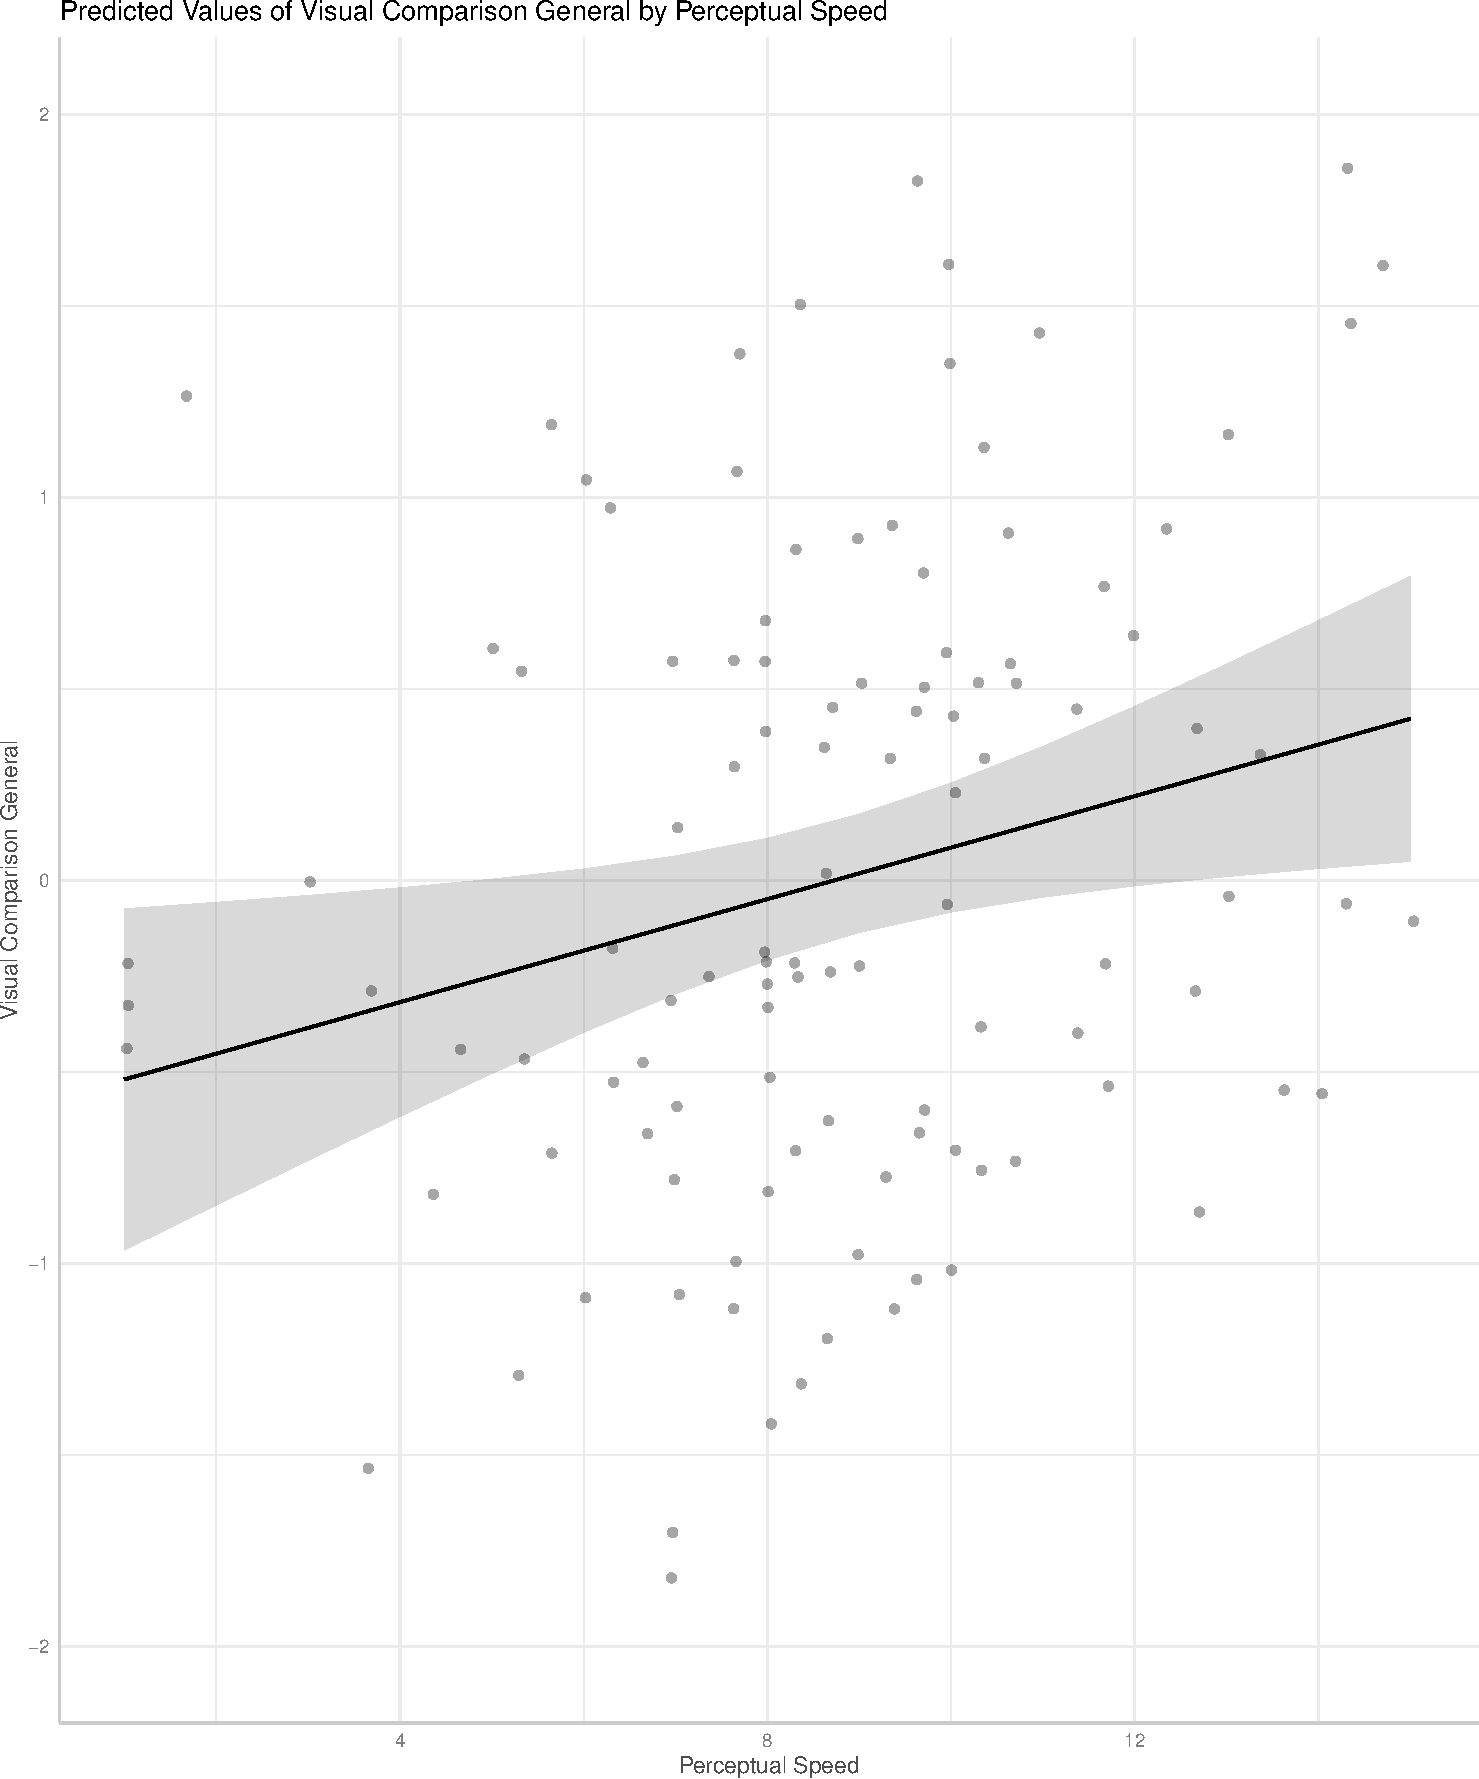
\includegraphics{comments-on-b-murphy-thesis-by-jb_files/figure-pdf/fig-1_1-1.pdf}

}

\caption{\label{fig-1_1}Graph of Results}

\end{figure}%

\newpage{}

\subsection*{References}\label{references}
\addcontentsline{toc}{subsection}{References}

\phantomsection\label{refs}
\begin{CSLReferences}{1}{0}
\bibitem[\citeproctext]{ref-bulbulia_2024_experiments}
Bulbulia, J. A. (2024). Methods in causal inference part 4: Confounding
in experiments. \emph{Evolutionary Human Sciences}, \emph{6}.
\url{https://osf.io/preprints/psyarxiv/6rnj5}

\end{CSLReferences}



\end{document}
